\twocolumn[\begin{@twocolumnfalse}
	\chapter{Making a Keyboard Adaptor cable\hfill\difficulty{3}}
	 Some `New Old Stock' (NOS) NABU Personal Computers are being sold without keyboards. Keyboards for other NABU PCs have over the years been misplaced or have developed faults. To address these issues, the NABU Preservation Project has released a Keyboard Emulator\footnotemark. The Keyboard Emulator software, in combination with a USB to RS-422 interface and a keyboard adaptor cable, allows NABU systems without keyboards to be controlled from a Windows PC. This section describes how to create the required DB-9 to DIN-6 keyboard adaptor cable.
	\vskip1em
\end{@twocolumnfalse}]
\footnotetext[1]{See the NABU RetroNet website <https://nabu.ca> for details.}

\section{Keyboard Adaptor cable wiring}
The \texttt{KEYBOARD} port on the back of the NABU Personal Computer implements a half-duplex RS-422 interface, which requires 2 wires for communication between devices. The cable must be connected as specified in Table~\ref{tbl:kbdadaptor}. For best performance, the adaptor cable should be kept as short as possible --- preferably less than 6 inches. Twisted-pair cable is highly recommended. To avoid a ground loop, only connect ground to either the DB-9 or DIN-6 connector, \textit{never both}.

\begin{center}
	\sffamily
	\begin{tblr}{
			colspec={r|cccc|},
			cell{1}{2} = {c=2}{c},
			cell{1}{4} = {c=2}{c},
			row{1} = {font=\bfseries},
			row{1,2} = {bg=gray4,fg=white},
			row{5,6} = {bg=gray9},
			cell{1}{1} = {r=2}{bg=white},
			cell{3}{1} = {r=2}{},
			cell{5}{1} = {r=2}{},
			vline{4} = {3-4}{text=\clap{$\leftrightarrow$}},
			vline{1} = {3-4}{solid},
			hline{1} = {2-5}{solid},
			hline{3,5} = {solid}
		}
		& NABU (DIN6) & & RS-422 (DB9)\footnotemark[2] &\\
		& Signal & Pin & Pin & Signal \\
		\rotatebox{90}{Pair} & T/R+ & 4 & 1 & T/R+ \\
		& T/R-- & 5 & 2 & T/R-- \\
	\end{tblr}
	\taskLbl{tbl:kbdadaptor}
	\taskTable{Adaptor cable wiring.}
\end{center}
\footnotetext[2]{Pin numbers shown are for the DTECH DT-5019 USB TO RS485/422 adaptor cable.  Refer to the relevant manufacturer's documentation for other RS-422 interfaces.}

\section{DIN-6 end of the cable}
\begin{enumerate}
	\item Solder the pins of a \underline{male} DIN-6 connector as shown in Figure \ref{fig:din6}. Note that the pin numbers shown in the diagram are for the solder side of the connector.
\end{enumerate}

\section{DB-9 end of the cable}
\begin{enumerate}
	\item Solder the pins on the \underline{female} DB-9 connector as shown in Figure \ref{fig:db9-kbd}.  Note that the pin numbers shown in the diagram are for the solder side of the connector.\\
	Alternatively, use a DB-9 adaptor with screw terminals, as shown in Figure \ref{fig:db9adapt-kbd}.
\end{enumerate}
\newpage
\begin{figure}[h!]
	\begin{center}
		\scalebox{0.175}{
			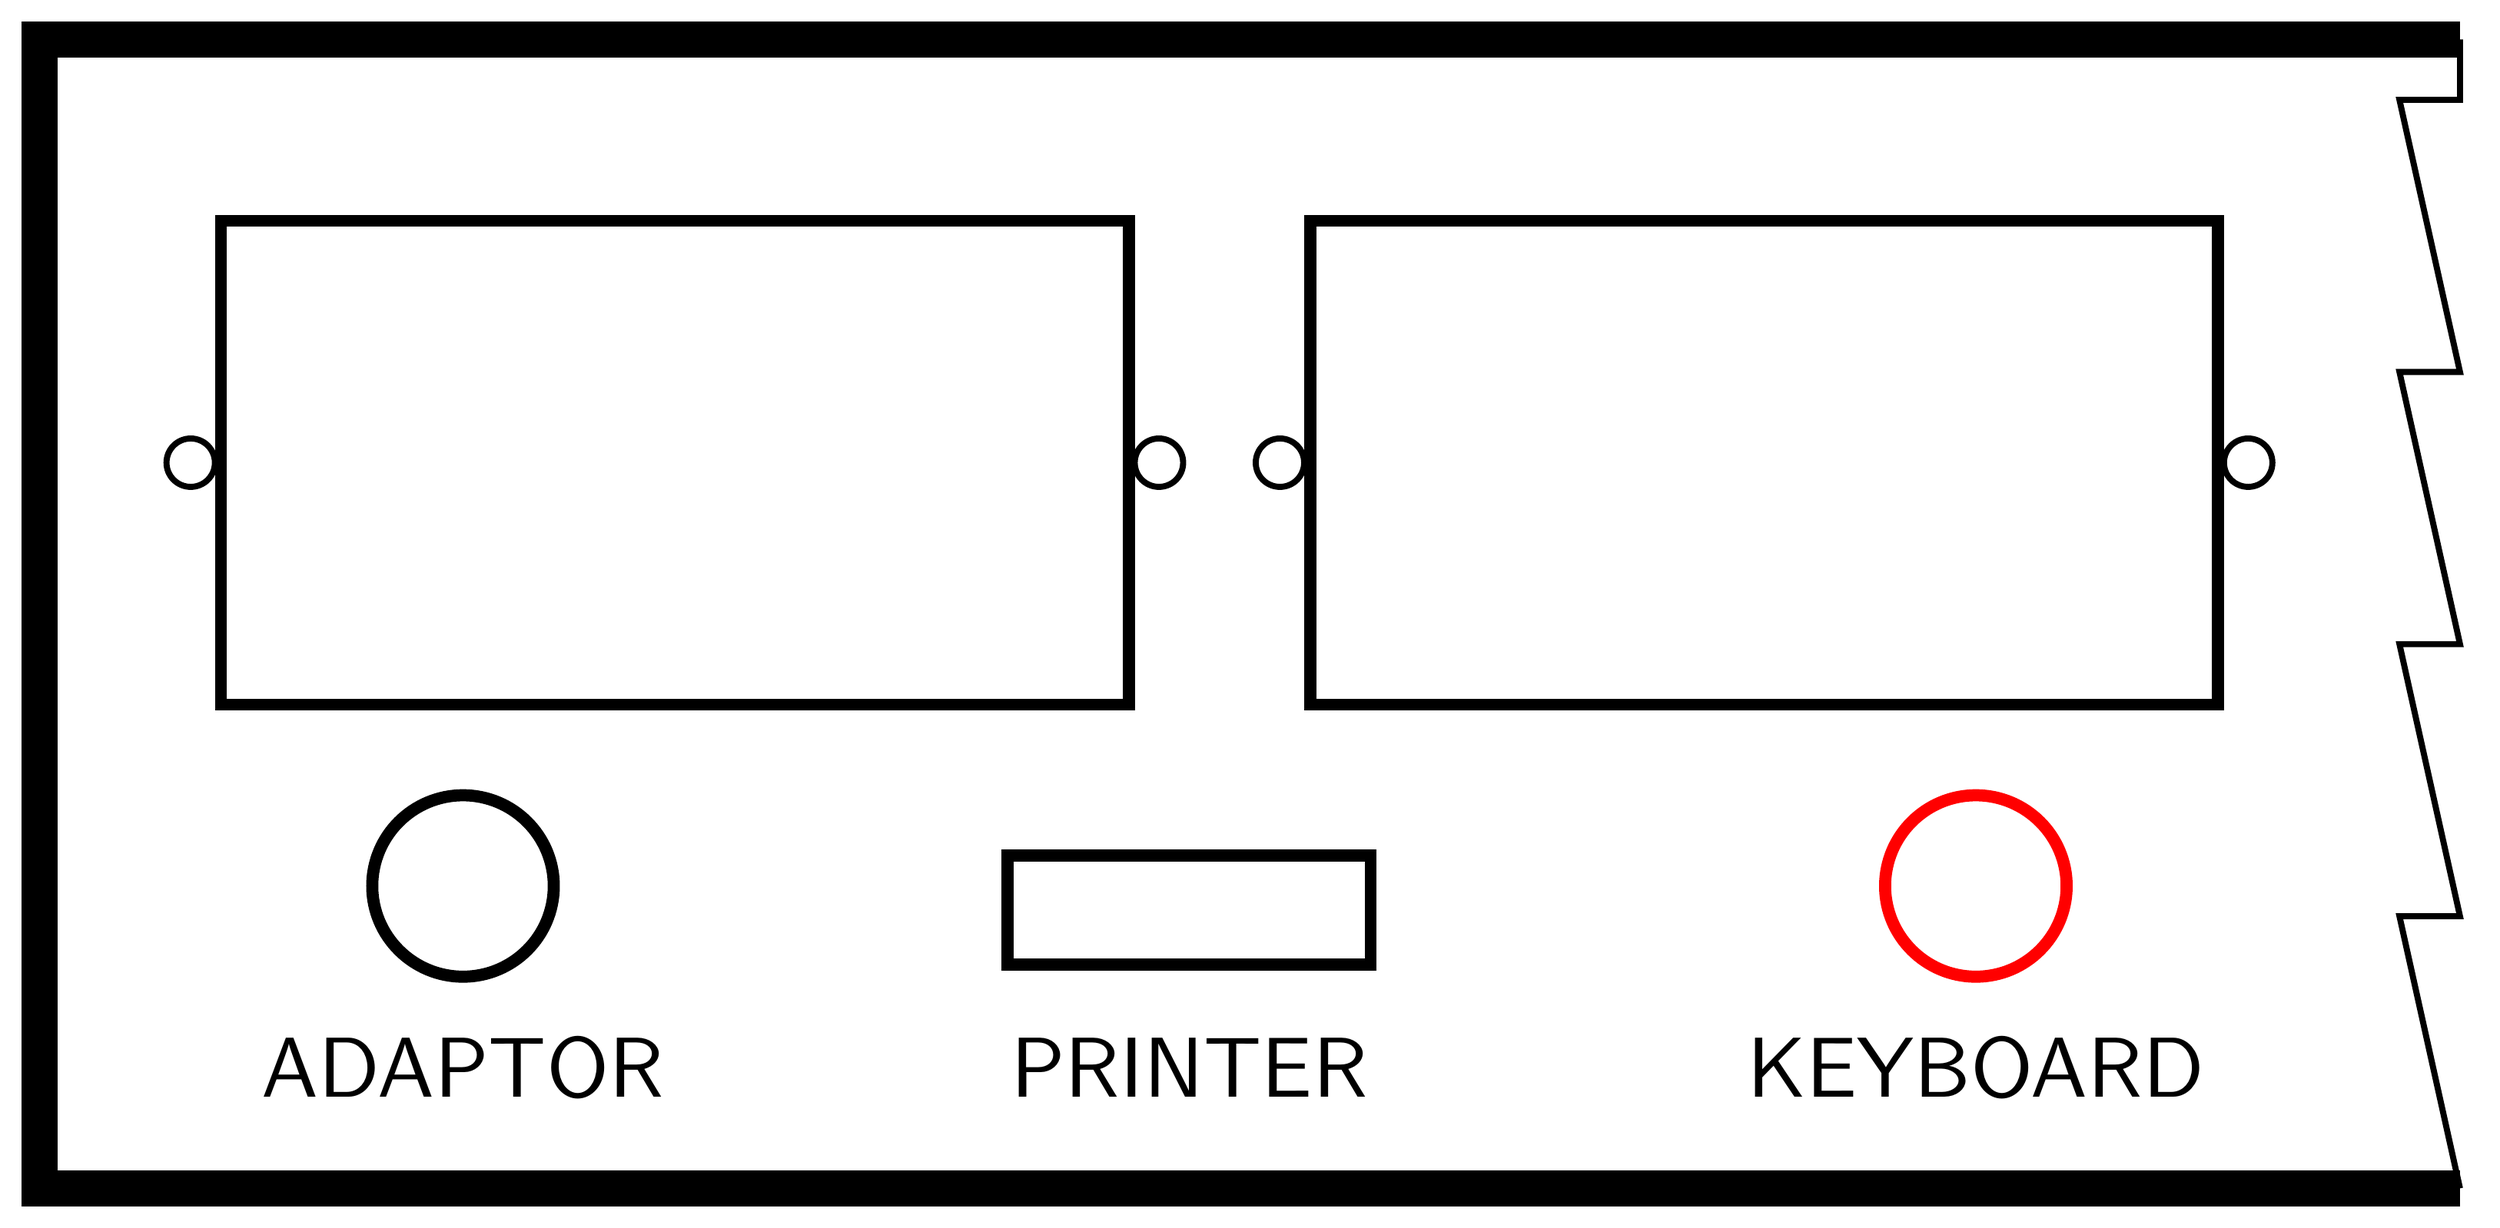
\begin{tikzpicture}[font=\sffamily]
				\draw[line width=6mm] (40,19) -- ++(-40,0) -- ++(0,-19) -- ++(40,0);
				\draw[line width=1mm,decorate,decoration={saw,segment length=45mm,amplitude=10mm}] (40,0) -- ++(0,19);
				\draw[line width=2mm,fill=white] (3,8) rectangle (18,16);
				\draw[line width=2mm,fill=white] (21,8) rectangle (36,16);
				\draw[line width=1mm,fill=white] (2.5,12) circle (4mm);
				\draw[line width=1mm,fill=white] (18.5,12) circle (4mm);
				\draw[line width=1mm,fill=white] (20.5,12) circle (4mm);
				\draw[line width=1mm,fill=white] (36.5,12) circle (4mm);

				\draw[line width=2mm,fill=white] (7,5) circle (15mm);
				\draw[line width=2mm,color=red,fill=white] (32,5) circle (15mm);
				\node[black,scale=4] at (7,2) {ADAPTOR};
				\node[black,scale=4] at (32,2) {KEYBOARD};
				\draw[line width=2mm,fill=white] (16,3.7) rectangle (22,5.5); \node[black,scale=4,] at (19,2) {PRINTER};
			\end{tikzpicture}
		}
		\caption[Keyboard port position.]{NABU Personal Computer \texttt{KEYBOARD} port.}
		\label{fig:backkbd}
	\end{center}
\end{figure}

\begin{figure}[h!]
	\begin{center}
		\scalebox{0.175}{
			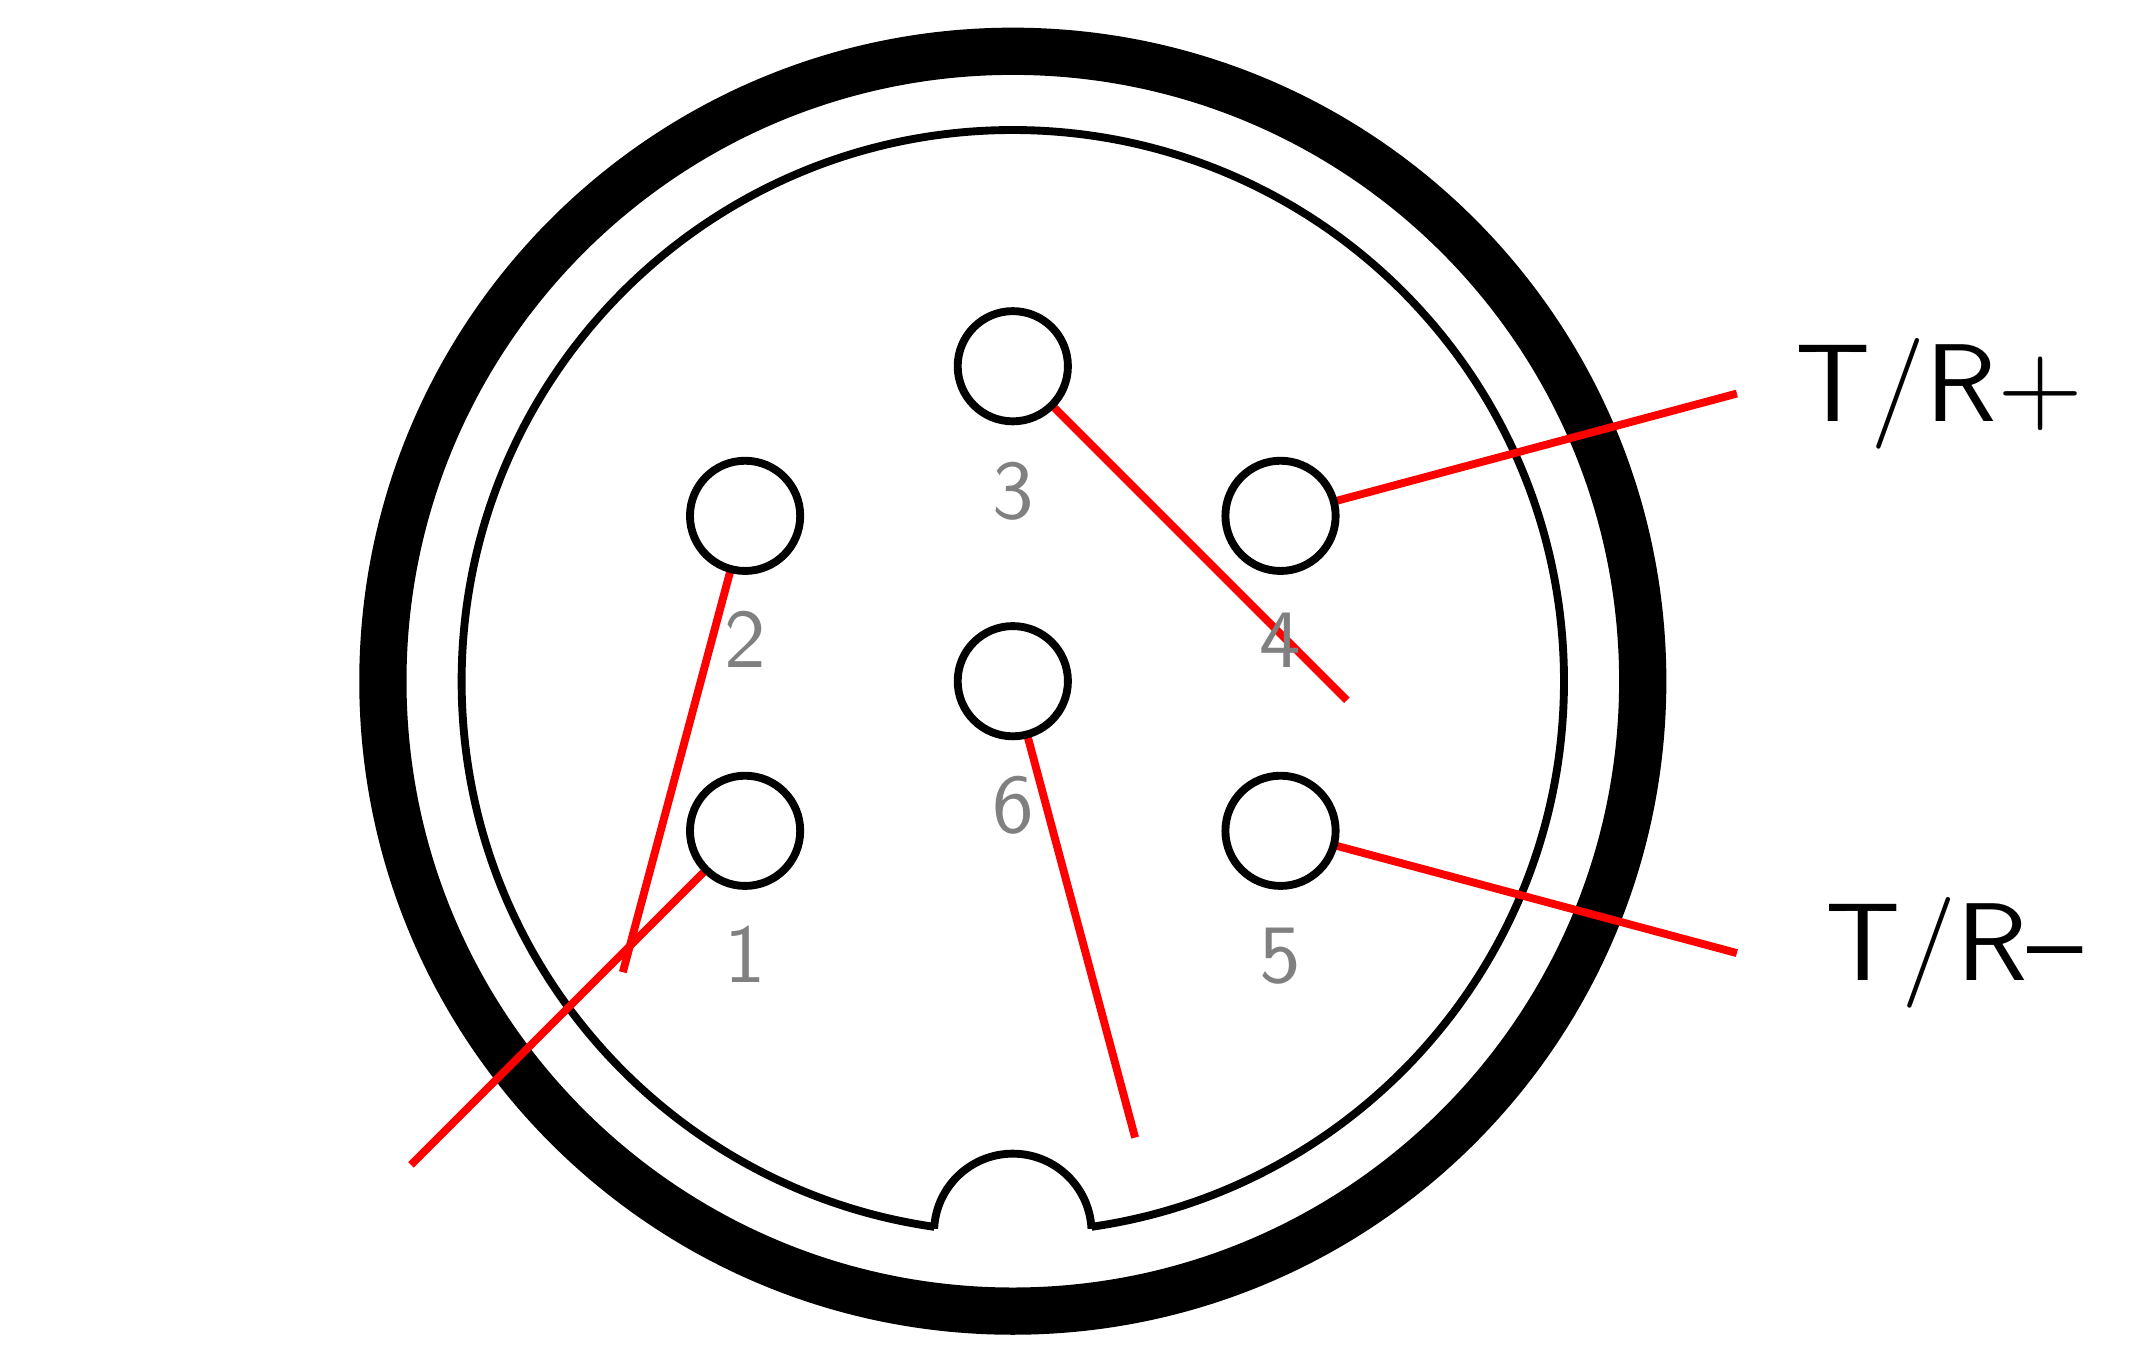
\begin{tikzpicture}[font=\sffamily]
				\draw[line width=6mm] (10,10) circle (8cm);
				\draw[line width=1mm] (10,10) circle (7cm);
				\fill[fill=white] (9,3.5) rectangle (11,2.8);
				\begin{scope}
					\clip (8.8,3.05) rectangle (11.2,6);
					\draw[line width=1mm] (10,3) circle (1cm);
				\end{scope}
				\foreach \p\k\m\n [count=\q from 1] in {
					{}/1/6.6/8.1,{}/2/6.6/12.1,{}/6/10/10,
					{}/3/10/14,{T/R--}/5/13.4/8.1,{T/R+}/4/13.4/12.1}
				{
					\ifthenelse{\q>4}{
						\pgfmathsetmacro{\r}{\q*30+-165}
						\draw[line width=1mm,red] (\m,\n) -- ++(\r:6cm) node[black,scale=4,text width=2.2cm,align=right]{\p};
					}{}
					\draw[line width=1mm,fill=white] (\m,\n) circle (7mm) node[scale=3,gray,yshift=-1.5em]{\k};
				}
			\end{tikzpicture}
		}
		\caption[DIN-6 male connector pinouts.]{DIN-6 male connector (solder side).}
		\label{fig:din6}
	\end{center}
\end{figure}

\begin{figure}[h!]
  \begin{center}
	\scalebox{0.2}{
		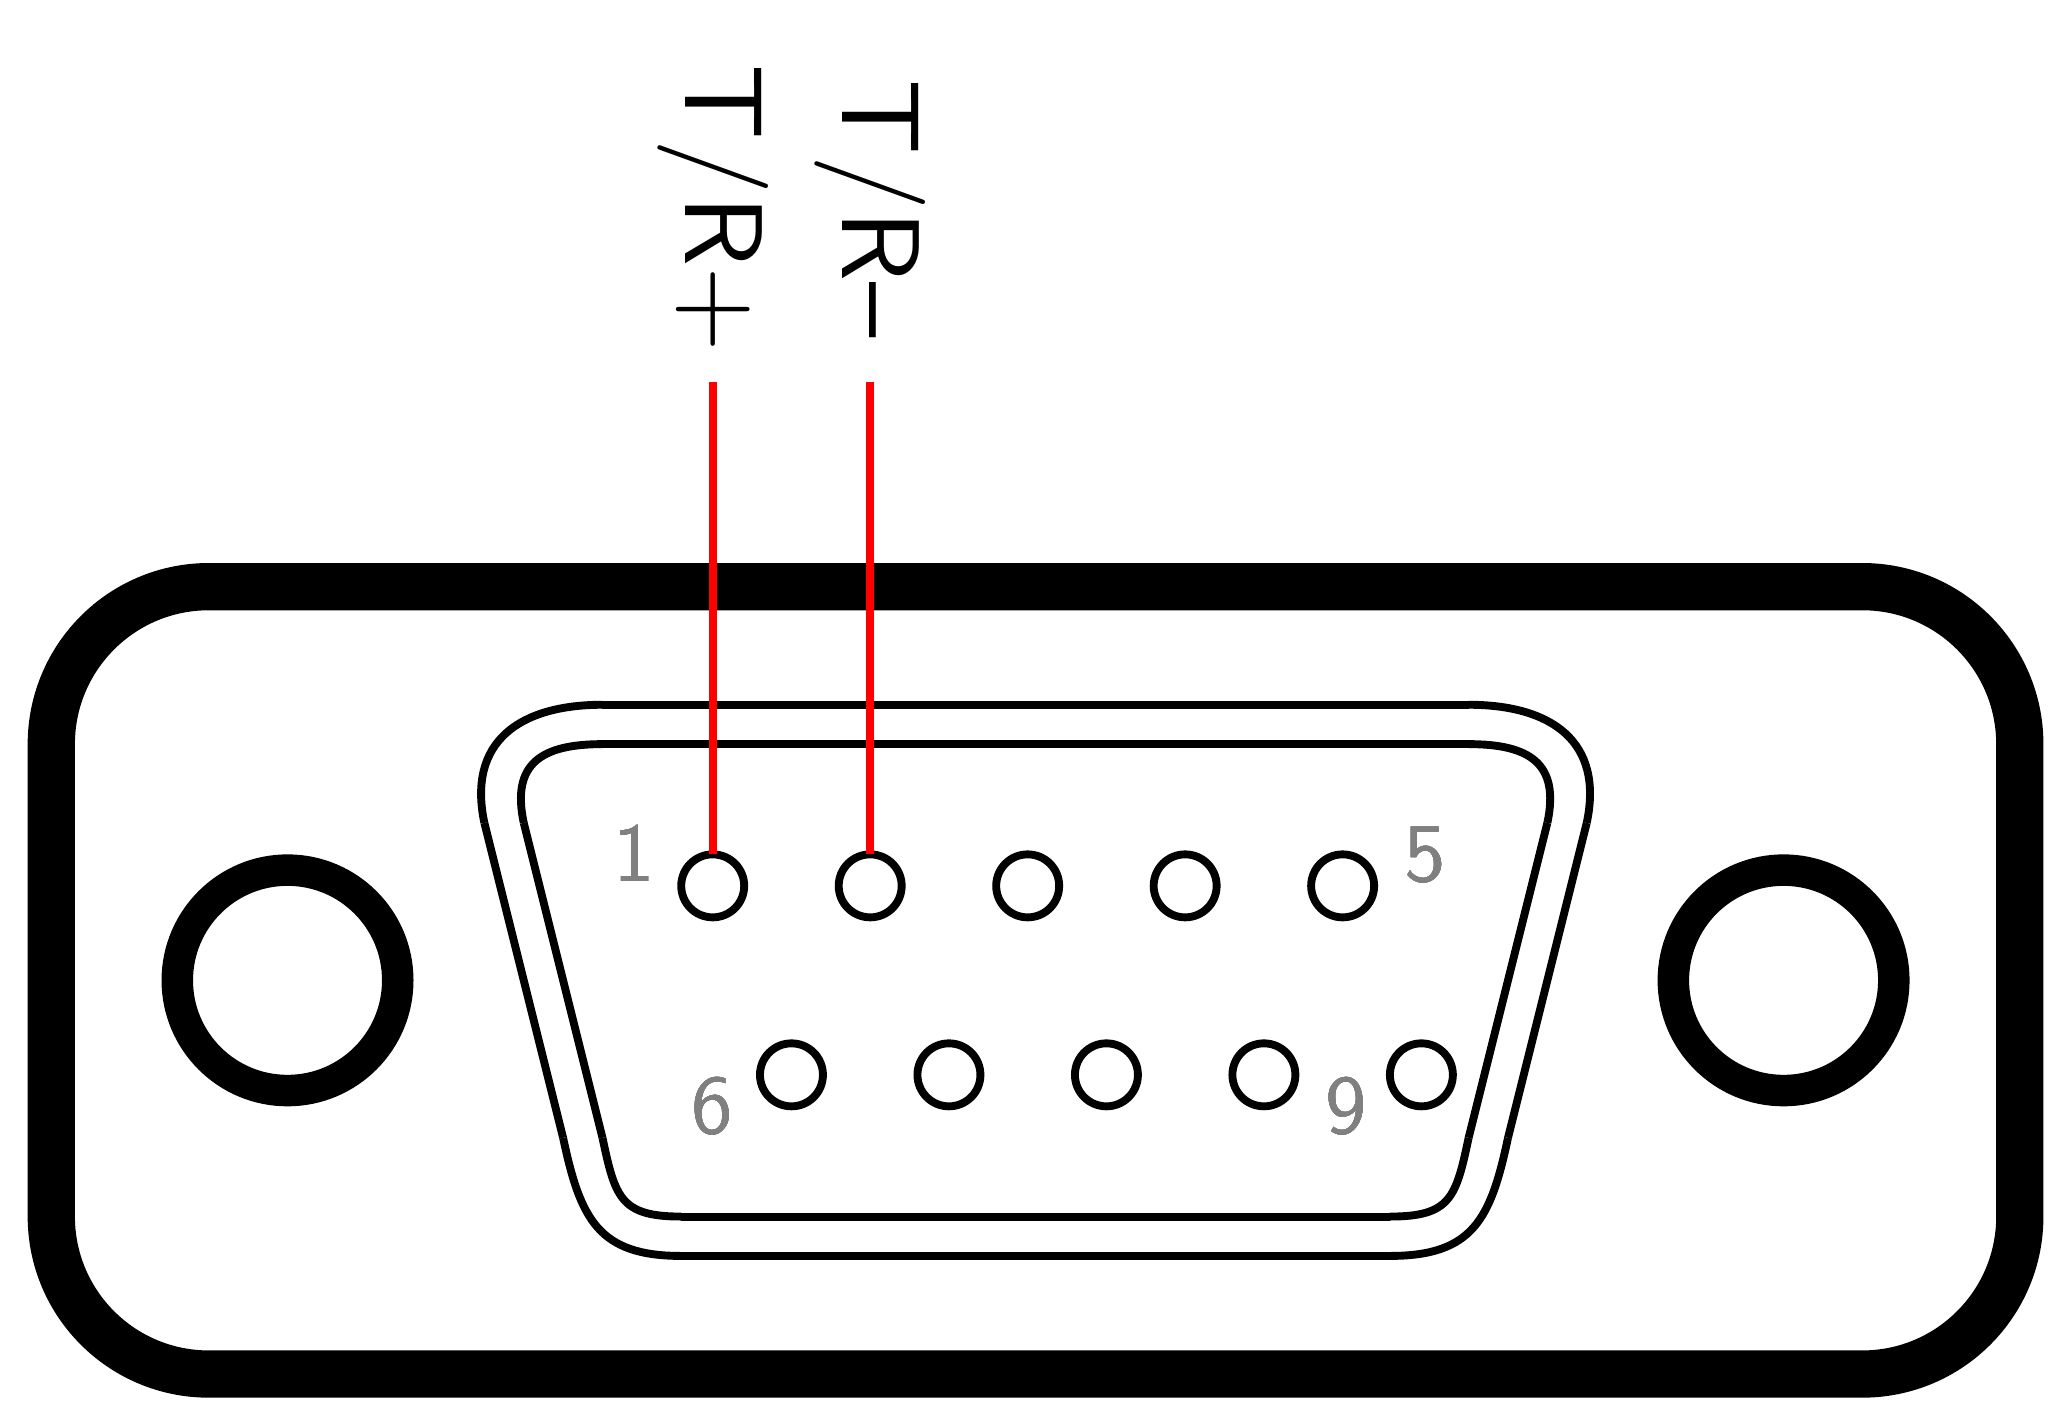
\begin{tikzpicture}[font=\sffamily]
			\draw[rounded corners=2cm,line width=6mm] (0, 0) rectangle (25,10) {};

			\draw[line width=4mm] (3,5) circle (1.4cm);
			\draw[line width=4mm] (22,5) circle (1.4cm);

			\draw[line width=1mm] (7,8) -- (18,8);
			\draw[line width=1mm] (8,2) -- (17,2);
			\draw[line width=1mm] (6,7) -- (7,3);
			\draw[line width=1mm] (19,7) -- (18,3);
			\draw[line width=1mm] (6,7) to[out=102,in=180,distance=22] (7,8);
			\draw[line width=1mm] (7,3) to[out=-78,in=180,distance=22] (8,2);
			\draw[line width=1mm] (17,2) to[out=0,in=-102,distance=22] (18,3);
			\draw[line width=1mm] (19,7) to[out=78,in=0,distance=22] (18,8);

			\draw[line width=1mm] (7,8.5) -- (18,8.5);
			\draw[line width=1mm] (8,1.5) -- (17,1.5);
			\draw[line width=1mm] (5.5,7) -- (6.5,3);
			\draw[line width=1mm] (19.5,7) -- (18.5,3);
			\draw[line width=1mm] (5.5,7) to[out=102,in=180,distance=30] (7,8.5);
			\draw[line width=1mm] (6.5,3) to[out=-78,in=180,distance=30] (8,1.5);
			\draw[line width=1mm] (17,1.5) to[out=0,in=-102,distance=30] (18.5,3);
			\draw[line width=1mm] (19.5,7) to[out=78,in=0,distance=30] (18,8.5);

			\foreach \p\k [count=\q from 0] in {{T/R+}/{},{T/R--}/{},{}/{},{}/{},{}/{}} {
				\draw[line width=1mm] (8.4+\q*2,6.2) circle (4mm);
				\ifthenelse{\q<4}{\draw[line width=1mm] (9.4+\q*2,3.8) circle (4mm);	}{}
				\foreach \x in \p {
					\draw[line width=1mm,red] (8.4+\q*2,6.6) -- ++(0,6);
					\draw (8.4+\q*2,14.8) node[rotate=-90,scale=4]{\p};
				}{}
				\foreach \x in \k {
					\draw[line width=1mm,red] (9.4+\q*2,3.4) -- ++(0,-6);
					\draw (9.4+\q*2,-4.8) node[rotate=-90,scale=4,text width=1cm]{\k};
				}
				\draw (7.4,6.6) node[scale=3,gray]{1};
				\draw (17.45,6.6) node[scale=3,gray]{5};
				\draw (8.4,3.4) node[scale=3,gray]{6};
				\draw (16.45,3.4) node[scale=3,gray]{9};
			}
		\end{tikzpicture}
	}
	\caption[DB-9 female connector pinouts.]{DB-9 female connector (solder side).$^2$}
	\label{fig:db9-kbd}
  \end{center}
\end{figure}

\begin{figure}[h!]
	\begin{center}
		\scalebox{0.19}{
			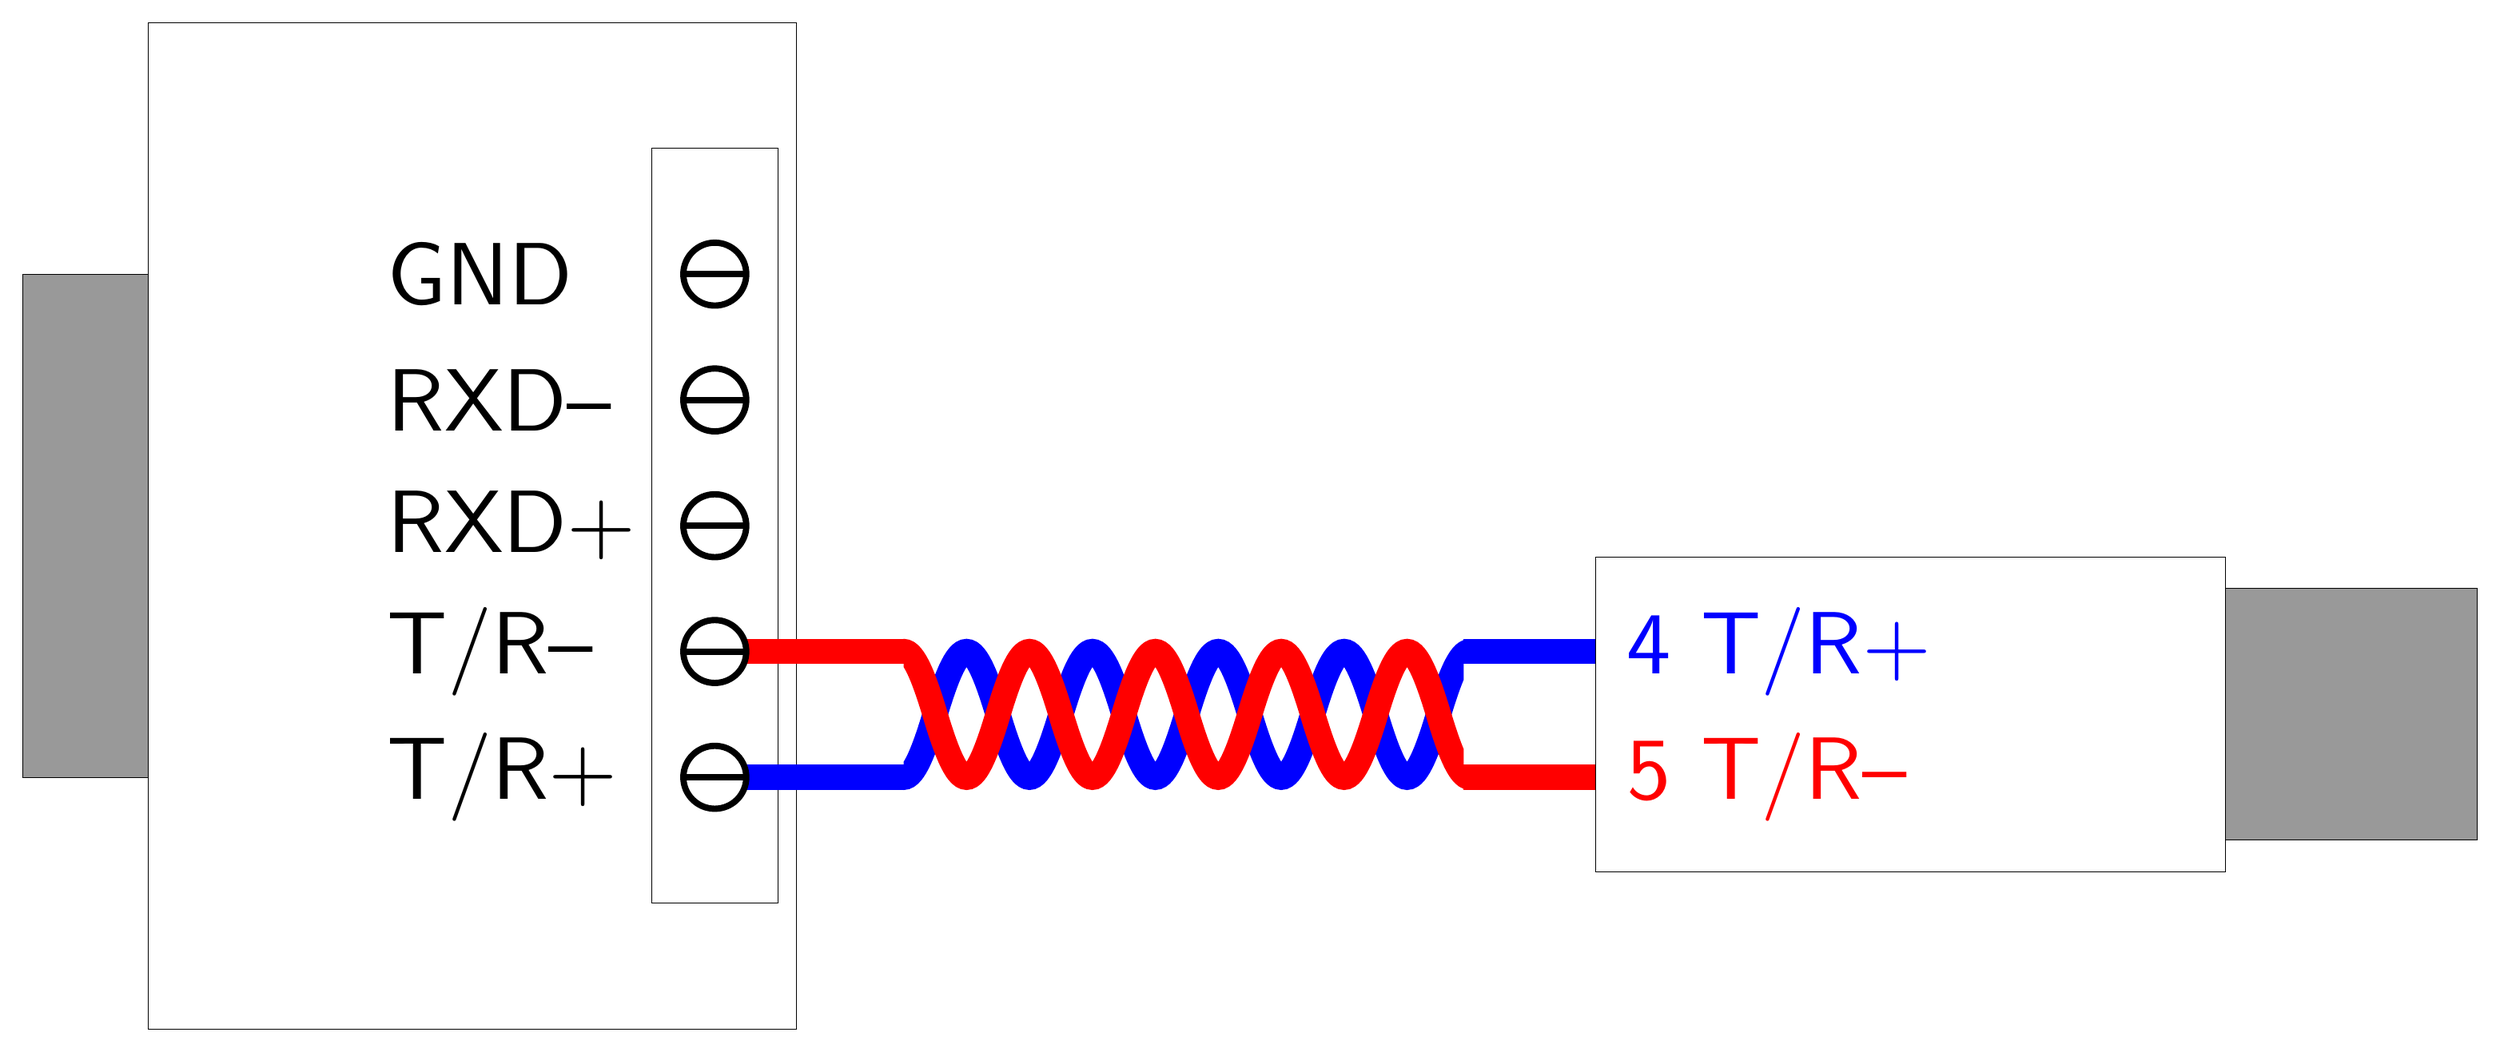
\begin{tikzpicture}[font=\sffamily]
				\draw[] (2,0) rectangle (12.3,16);
				\draw[] (10,2) rectangle (12,14);
				\draw[line width=4mm, color=red] (22.9,4) -- (25,4) node [scale=4,xshift=3.2em,text width=2cm] {5 T/R--};
				\draw[line width=4mm, color=red] (11,6) -- (14,6);
				\draw[line width=4mm, color=blue] (22.9,6) -- (25,6)  node [scale=4,xshift=3.2em,text width=2cm] {4 T/R+};
				\draw[line width=4mm, color=blue] (11,4) -- (14,4);
				\draw[fill=black!40] (0,4) rectangle (2,12);
				\foreach \k [count=\q from 0] in {{T/R+},{T/R--},{RXD+},{RXD--},{GND}}{
					\draw[line width=1mm,fill=white] (11,\q*2+4) circle (5mm);
					\draw[line width=1mm] (11.5,\q*2+4) -- ++(-1,0) node [scale=4,xshift=-.5em,text width=2cm, align=left] {\k};
				}
				\draw[fill=black!40] (35,3) rectangle (39,7);
				\draw[] (25,2.5) rectangle (35,7.5);

				\begin{scope}
					\clip(14,2) rectangle (22.9,7);
					\draw[line width=4mm,color=blue,decorate,decoration={coil,aspect=0, amplitude=10mm,segment length=20mm}] (12.5,5) -- (23.6,5);
					\draw[line width=4mm,color=red,decorate,decoration={coil,aspect=0, amplitude=10mm,segment length=20mm}] (23.5,5) -- (12.2,5);
				\end{scope}
			\end{tikzpicture}
		}
	\caption[DB-9 adaptor terminals.]{DB-9 adaptor to DIN-6 wiring.$^2$}
	\label{fig:db9adapt-kbd}
	\end{center}
\end{figure}
